%%%%%%%%%%%%%%%%%%%%%%%%%%%%%%%%%%%%%%%%%
% a0poster Portrait Poster
% LaTeX Template
% Version 1.0 (22/06/13)
%
% The a0poster class was created by:
% Gerlinde Kettl and Matthias Weiser (tex@kettl.de)
% 
% This template has been downloaded from:
% http://www.LaTeXTemplates.com
%
% License:
% CC BY-NC-SA 3.0 (http://creativecommons.org/licenses/by-nc-sa/3.0/)
%
%%%%%%%%%%%%%%%%%%%%%%%%%%%%%%%%%%%%%%%%%

%----------------------------------------------------------------------------------------
%	PACKAGES AND OTHER DOCUMENT CONFIGURATIONS
%----------------------------------------------------------------------------------------

\documentclass[a0,portrait,20pt]{a0poster}

\usepackage{multicol} % This is so we can have multiple columns of text side-by-side
\columnsep=100pt % This is the amount of white space between the columns in the poster
\columnseprule=3pt % This is the thickness of the black line between the columns in the poster

\usepackage[svgnames]{xcolor} % Specify colors by their 'svgnames', for a full list of all colors available see here: http://www.latextemplates.com/svgnames-colors

\usepackage{times} % Use the times font
%\usepackage{palatino} % Uncomment to use the Palatino font

\usepackage{graphicx} % Required for including images
\graphicspath{{figures/}} % Location of the graphics files
\usepackage{booktabs} % Top and bottom rules for table
\usepackage[font=small,labelfont=bf]{caption} % Required for specifying captions to tables and figures
\usepackage{amsfonts, amsmath, amsthm, amssymb} % For math fonts, symbols and environments
\usepackage{wrapfig} % Allows wrapping text around tables and figures
\usepackage[labelformat=empty]{caption}

\begin{document}

%----------------------------------------------------------------------------------------
%	POSTER HEADER 
%----------------------------------------------------------------------------------------

% The header is divided into two boxes:
% The first is 75% wide and houses the title, subtitle, names, university/organization and contact information
% The second is 25% wide and houses a logo for your university/organization or a photo of you
% The widths of these boxes can be easily edited to accommodate your content as you see fit

\begin{minipage}[b]{0.75\linewidth}
\veryHuge \color{NavyBlue} \textbf{CATMANIA} \color{Black}\\ % Title
\Huge\textit{A study of international fictional cats.}\\[2cm] % Subtitle
\huge \textbf{Quitterie \textsc{Cazenave}, Segolene \textsc{Tubau} \& Guilhem \textsc{Saurel}}\\[0.5cm] % Author(s)
\huge INP-ENM \& INP-ENSEEIHT\\[0.4cm] % University/organization
\end{minipage}
%
\begin{minipage}[b]{0.25\linewidth}

\includegraphics[width=20cm]{logo.png}\\
\end{minipage}

\vspace{1cm} % A bit of extra whitespace between the header and poster content

%----------------------------------------------------------------------------------------

\begin{multicols}{2} % This is how many columns your poster will be broken into, a portrait poster is generally split into 2 columns

%----------------------------------------------------------------------------------------

\color{SaddleBrown} % SaddleBrown color for the introduction

\section*{Introduction}

\begin{wrapfigure}[9]{l}{6cm}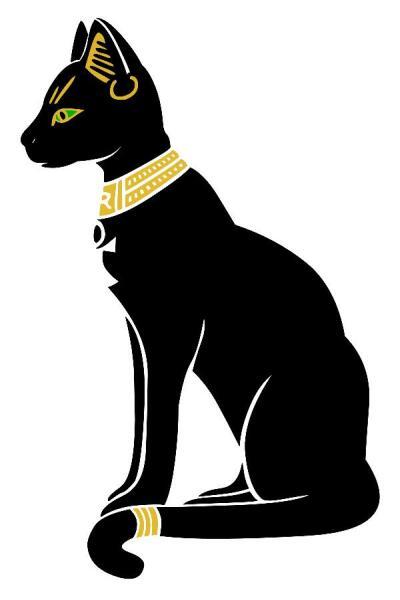
\includegraphics[width=6cm]{bastet.png}\caption{Bastet}\end{wrapfigure}
\large We can see them everywhere on the internet. They were venerated back in the ancient time as it was the case in Egypt. Some of them even received the same mummification after death as humans. Why are cats that popular? How can we explain that ever after several millennia they are still so popular among us?

~

In the ancient time cats were domesticated because they could kill unwanted living beings such as rats or snakes. Thanks to this fact they were praised for controlling vermin and became a symbol of grace and poise. Since then they succeeded in becoming indispensable in our society. Nowadays cats are little ball of fur that are living with us as pets.


%----------------------------------------------------------------------------------------

\color{DarkSlateGray} % DarkSlateGray color for the rest of the content

\section*{Fictional Cats in Asia}

\begin{wrapfigure}[6]{l}{6cm}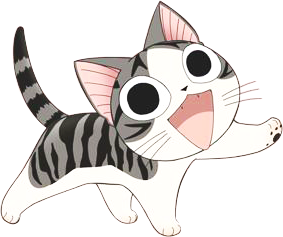
\includegraphics[width=6cm]{a1.png}\caption{Chi}\end{wrapfigure}
In Asia, people are so fond of cats that they became a large phenomenon. They find them cute with their sweet eyes, funny when they are playing and mischievous when they pull pranks on people. All these aspects make them look adorable in our eyes. That why Asian people consider cats as the cutest pet. However, there are more qualities to see in them than just the previous ones. A cat is a creature that behaves with elegance. Their demeanour, the way it moves silently, graciously and nimbly make people consider cats as cool living being. All this explain why sometime cats are seen as cool and stylish.

~

\begin{wrapfigure}[5]{r}{6cm}
\includegraphics[width=6cm]{a2.png}\end{wrapfigure}
Since everything that is popular in Asia can be seen in manga, it is naturally the case with cats. Thus we can see cats in a lot of mangas. There in even mangas in which we can follow the adventures of cats such as the manga named Chi’s sweet home. In this manga, we can read the life of Chi, a funny and clumsy kitten. Cats are also used as mascots in some stories. As an illustration, in Fairy Tail we can see “exceed”, a race of cat-like beings that can use magic in order to get wings and fly.

~

\begin{wrapfigure}[6]{l}{6cm}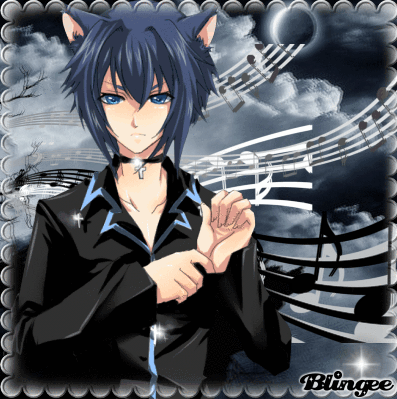
\includegraphics[width=6cm]{a3.png}\end{wrapfigure}
Moreover, the popularity of cats is so considerable that we can say that there is currently a “cat phenomenon” in Japan. The matchless success of Hello Kitty in Japan and the figurine of the  cat version of a lot of manga characters are signs that confirm this fact. There is even what we can call a cat type of character in manga. On the one hand we can see playful and mischievous characters with a cat-like behaviour such as wanting to catch something moving near them or saying “nya” (the Japanese word equivalent to the English word “meow”) at the end of each of their sentences. On the other hand there are distant and cool characters moving nimbly and gracefully as a cat. In all of these two cat-like kind of character, some have got cat ears or hairstyle such as it seem as they have cat ears.


%----------------------------------------------------------------------------------------

\section*{Fictional Cats in Europe}

In the european litterature as in our lives and beliefs, cats have always had a prominent place. Through its representation in european comics we can make a list of the principal characteristics that we, human being, would describe a cat with.

~

\begin{wrapfigure}[4]{l}{6cm}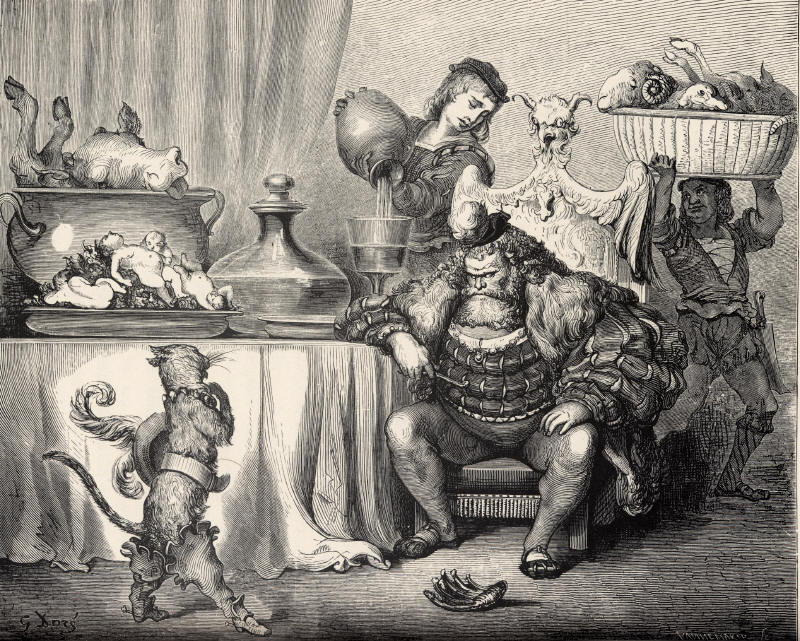
\includegraphics[width=6cm]{botte.jpg}\caption{Le Chat Botte}\end{wrapfigure}
Let’s start with an old tale: Le chat botte, from Charles Perrault where a cat comes wearing boots and helps a poor young man to become rich. In this tale, the cat appears clever and cunning, fooling and stealing men for his master.

~

\vspace{2cm}

\begin{wrapfigure}[8]{r}{6cm}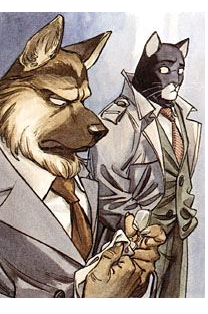
\includegraphics[width=6cm]{blacksad.png}\caption{Blacksad}\end{wrapfigure}
The cleverness of the cat is also described in Blacksad, from Canales and Guranido where the main character is represented as a cat private detective. In this comic, all the characters are manlike animals. The character of John Blacksad is also represented as solitary and nostalgic. Whereas, for example, the policeman also in charge with the case is a dog and is represented as honest, straight and, upright. As they are a cat and a dog, there is also a rivalry between the two.

~


\begin{wrapfigure}[6]{l}{6cm}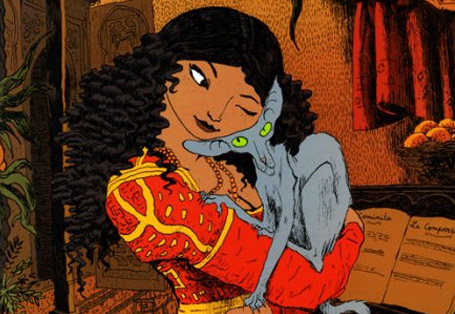
\includegraphics[width=6cm]{rabin.jpg}\caption{Le Chat du Rabbin}\end{wrapfigure}
Le chat du rabbin from Joann Sfar: a magic (or holy) and mysterious cat: he can talk but nobody knows why + to describe the humans from a different perspective, the one of a different being who shares our everyday life.

From all the animals living close to us, it is also the one that looks the most like us: his rather flat face, his cleverness.

~

\begin{center}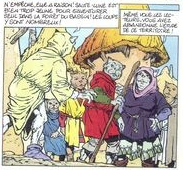
\includegraphics[width=6cm]{chats.png} \\ Chats, from Convard\end{center}

~

\begin{center}
    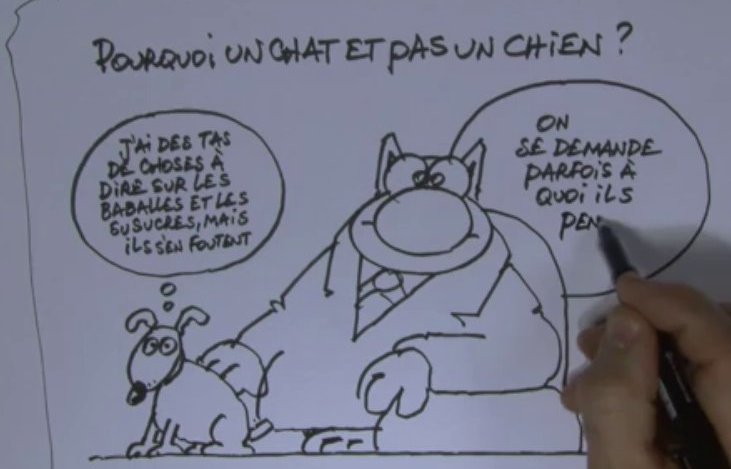
\includegraphics[width=6cm]{chat.png}

    Le Chat, from Geluck: he is a cat but he looks like a human and behave like a human.
\end{center}

~

\begin{wrapfigure}[3]{r}{6cm}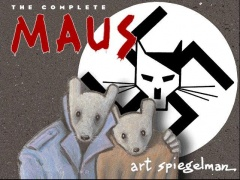
\includegraphics[width=6cm]{maus.jpg}\caption{Maus}\end{wrapfigure}
Maus : cruelty of the carnivorous chasing the mouse to represent the Nazi hunting and exterminating the Jews. It deals with a difficult subject keeping a distance to make it easier.

\vspace{2.5cm}

%----------------------------------------------------------------------------------------

\section*{Fictional Cats in America}

\begin{wrapfigure}[6]{l}{6cm}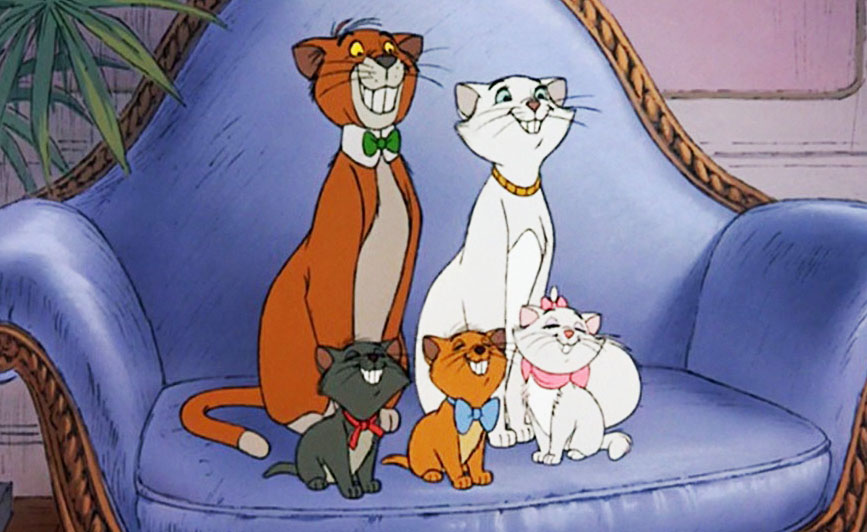
\includegraphics[width=6cm]{aristo.png}\caption{The Aristocats}\end{wrapfigure}
In 1910 lived a rich woman, without any heir. She decided to left her fortune to her cat Duchesse and its three kittens, Marie, Berlioz and Toulouse.

~

Of course, the butler wants that fortune, and set up a plan to leave the cats into the countryside.

~

\begin{wrapfigure}[5]{r}{6cm}
\includegraphics[width=6cm]{tom.png}\caption{Tom \& Jerry}\end{wrapfigure}
Tom and Jerry has the simplest plot : the fight between a house cat and a mouse.

~

Most of the time, Jerry wins, making fun of Tom, but sometimes they have to cooperate for a common goal.

~

\begin{wrapfigure}[5]{l}{6cm}
\includegraphics[width=6cm]{felix.png}\caption{Felix the cat}\end{wrapfigure}
Felix the cat began as a very popular serie of shorts. 183 animated films have been made in 19 years, and some of them are in the public domain, and therefore freely available on the internet (http://archive.org).

~

\begin{wrapfigure}[5]{r}{6cm}
\includegraphics[width=6cm]{garfield.png}\caption{Garfield}\end{wrapfigure}
Garfield is a house cat which is excessively lazy, eats obsessively and disdains work, mondays, exercise and diets.

Garfield is also pessimistic, sadistic, cynical, sarcastic, sardonic and a bit obnoxious.

~

\begin{wrapfigure}[5]{l}{6cm}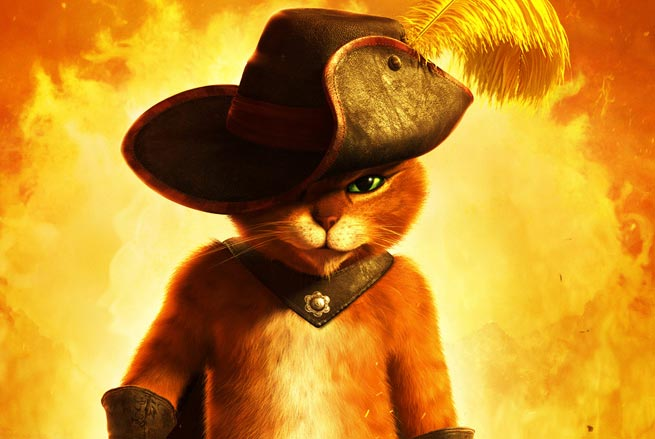
\includegraphics[width=6cm]{puss.png}\caption{Puss in Boots}\end{wrapfigure}
Based on Charle Perrault's fairy tale, this character first appeared in Shrek 2, and It now owns an eponym spin-off prequel.

Voiced by and based on Antonio Banderas, its catness stays representated by a lot of different feline gags.

~

\begin{wrapfigure}[5]{r}{6cm}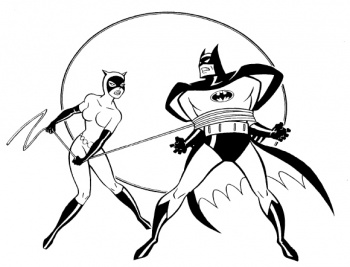
\includegraphics[width=6cm]{catwoman.png}\caption{Catwoman}\end{wrapfigure}
Catwoman began as a supervillain against Batman ; but she is now known to have a complex love-hate relationship with him.

She mainly wears black tight leather and fight with a whip and artificial claws, so her sadomasochist appearance and gadgets helps to understand this relation.
%----------------------------------------------------------------------------------------

~

\begin{center}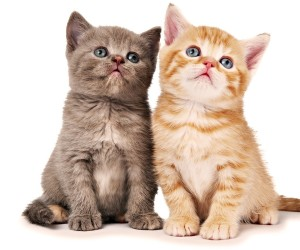
\includegraphics[width=6cm]{chattons.png}\end{center}
%----------------------------------------------------------------------------------------

\end{multicols}
\end{document}
